\section{Experiment 8F: deployment robustness of private federated LPV estimation}
\label{sec:experiment8f}

\paragraph{Question.}
Experiment 8F tests deployment effects omitted from Experiments 8C--8E:
partial participation, imperfect public clipping bounds, bounded outlying
contributions, and reduced tire--road friction. It replaces Experiment 8E's
arbitrary 15\% improvement criterion with an operational quantity: the minimum
cohort that keeps tracking degradation from its matching non-private aggregate
at or below 10\%.

\paragraph{Frozen protocol and gate.}
Ten fresh training fleets (seeds 96--105) contain 100 clients per family, with
separate nonlinear ten-client test fleets. Cohorts
$n\in\{10,20,30,50,100\}$ are selected by balanced, random, or deliberately
low-speed-biased policies. Isotropic and public control-aware mechanisms retain
replacement adjacency, $\delta=10^{-5}$, and
$\epsilon\in\{2,4,8,\infty\}$; common random draws enable paired comparisons.
A cell is viable when tracking cost is at most 10\%, every nonlinear run is
amplitude-feasible, and the worst frozen radius is below one.

Stage B fixes three $\epsilon=4$ points: $n=10$ (nonviable), $n=30$
(boundary), and $n=100$ (viable). It repeats them with the correct box, a box
narrowed by 10\%, a box shifted upward by 5\%, and 5\% or 10\% bounded outlier
contributions, at friction coefficients $\mu=0.9$ and $0.7$. The deployment
gate requires the viable point to pass all stresses. Outliers are adversarial
aggregation inputs projected by the mechanism, not new physical vehicle models.

\begin{table}[htbp]
\centering
\caption{Minimum viable cohort. All participation policies give the same minima.}
\label{tab:experiment8f-cohort}
\begin{tabular}{rrrr}
\toprule
$\epsilon$ & Isotropic & Control-aware & Cohort reduction\\
\midrule
2 & 100 & 100 & 0\%\\
4 & 50 & 50 & 0\%\\
8 & 30 & 20 & 33.3\%\\
\bottomrule
\end{tabular}
\end{table}

\begin{table}[htbp]
\centering
\caption{Tracking-cost ranges across both friction levels and all five stresses
at $\epsilon=4$.}
\label{tab:experiment8f-stress}
\begin{tabular}{lrrc}
\toprule
Point & Isotropic & Control-aware & All viable\\
\midrule
$n=10$ nonviable & 82.05--104.54\% & 63.28--81.74\% & no\\
$n=30$ boundary & 14.86--19.99\% & 10.67--14.33\% & no\\
$n=100$ viable & 0.18--2.02\% & $-0.04$--1.51\% & yes\\
\bottomrule
\end{tabular}
\end{table}

\begin{figure}[htbp]
\centering
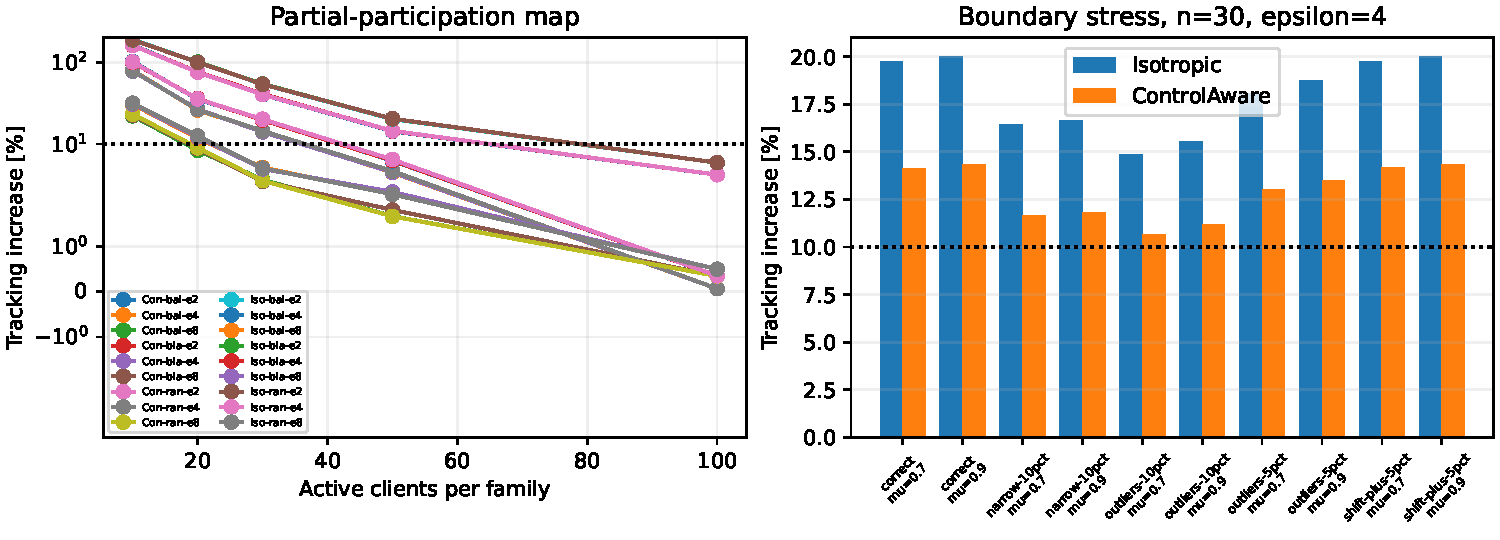
\includegraphics[width=0.93\linewidth]{../results/figures/experiment_8f_deployment_robustness.pdf}
\caption{Minimum viable cohort and deployment-stress results under the fixed
10\% tracking-cost boundary.}
\label{fig:experiment8f}
\end{figure}

\paragraph{Results.}
All 3,000 local fits converge. The experiment evaluates 25,200 private releases
and 756,000 nonlinear client--scenario combinations. All closed-loop runs are
amplitude-feasible and the largest frozen radius is below one. Minimum cohort is
insensitive to the tested participation policies. For control-aware privacy it
is 100, 50, and 20 at $\epsilon=2,4,8$; isotropic privacy requires 100, 50, and
30. Hence shaping reduces the required cohort by one third at $\epsilon=8$.

At $n=100,\epsilon=4$, both mechanisms pass every Stage B stress. Their largest
tracking costs are 2.02\% (isotropic) and 1.51\% (control-aware), including at
$\mu=0.7$. Neither mechanism makes the $n=30$ or $n=10$ point viable under all
stresses, preserving the boundary of the supported region. In total 16,224
released coordinates are projected to a public box, so clipping is active.

\paragraph{Interpretation and limitations.}
Experiment 8F passes its deployment gate. The supported claim is an empirical
cohort--privacy operating region that remains valid under the stated bounded
perturbations. Control-aware shaping reduces cohort size in one regime; it is
not universally superior. The participation finding is benchmark-specific,
the outlier test is not Byzantine security, and privacy covers one release
rather than repeated-round composition.

\paragraph{Reproducibility.}
The design is in \path{code/config/experiment_8f.json}; the runner is
\path{code/experiments/experiment_8f_deployment_robustness.py}. Friction is
propagated by \path{code/experiments/experiment_6b_acceleration_validation.py}.
Aggregate and seed-level evidence is retained under \path{results/tables}.
